\documentclass{report}

\usepackage{graphicx}
\usepackage{hyperref}
\usepackage{tikz}
\usepackage{pgfplots}
\usepackage{multirow}
\usepackage{tabulary}


\author{Mihalache Radu-Stefan}
\date{}
\title{Study of functions using Hill Climbing and Simulated Annealing algorithms}



\begin{document}
\maketitle

\section{Abstarct}
Analyzing Simulated Annealing and Hill Climbing algorithms to evaluate mathematical functions on multiple dimensions and find the minimum point on specific intervals.

\section{Introduction}
\subsection{Motivation}
The problem of exploring the values of functions and finding the global minimum of said function for a specified domain has useful aplications, yet it is dificult to solve with a deterministic algorithm.
That is because some functions have a very steep path to the minimum, like in the example below.

\begin{figure}[!h]
  \centering
\begin{tikzpicture}
  \begin{axis}[
      xlabel=x,
      ylabel=$f(x)$
    ]
    \addplot [
      color=red,
      mark=x
    ]
    coordinates {
      (0, 5)
      (1, 5.1)
      (2, 5.2)
      (3, 5.3)
      (3.3, 0)
      (3.5, 5.4)
      (7, 5.5)
    };
  \end{axis}
\end{tikzpicture}
\end{figure}

\section{Method}

Nondeterministic algorithms can be used to overcome this problem, as they have a better chance to explore the function and find the minimum . 
\newline
The representation of the input variables will be a string of n bits such that they can accuately represent the function domain.

$$x = a + decimal_{represenation}(bit_{str}) \cdot (b - a)/(2^n - 1) ,  x \in \left[a, b \right]$$

Using this represenattion, a random input called candidate solution can be generated, and its vecinity can be explored by negating one bit, such that the hamming distance between the candidate solution and the vecinity is one. This leads to the following aproaches:
\newline
\newline
Hill Climbing:
\newline
\newline
Select a candidate solution for each iteration and try to improove it using either the first better vecinity or the best vecinity. This algorithm finds the minimumm by exploring the basin of the candidate solution.
\newline
\newline
Simulated annealing:
\newline
\newline
Select a candidate solution at the start and explore its vecinity. This algorithm better explores the domain of the function by choosing worse vecinities base on the probability given by this expression:
\newline
$$random.uniform(0, 1) < math.exp(-abs((evaln - evalc) / temperature))$$
\newline
This algorithm makes use of the hot iron concept. At the begining the temperature  is high and the chance to choose a worse solution is high but it decreeses over each iteration based on this formula:
\newline
$$temperature = temperature * 0.9$$


\section{Experiment}

For this experiment, a python program will analyse theese functions on 5, 10 and 30 dimensions with 100 iterations and $10^{-5}$ precissionn. Each test is run 30 times to ensure consistancy

\begin{figure}[!h]
  \centering
  $$ f(x) = \sum_{i=1}^n \left[ x_i^2 \right],
   x_i \in \left[ -5.12, 5.15 \right]$$

  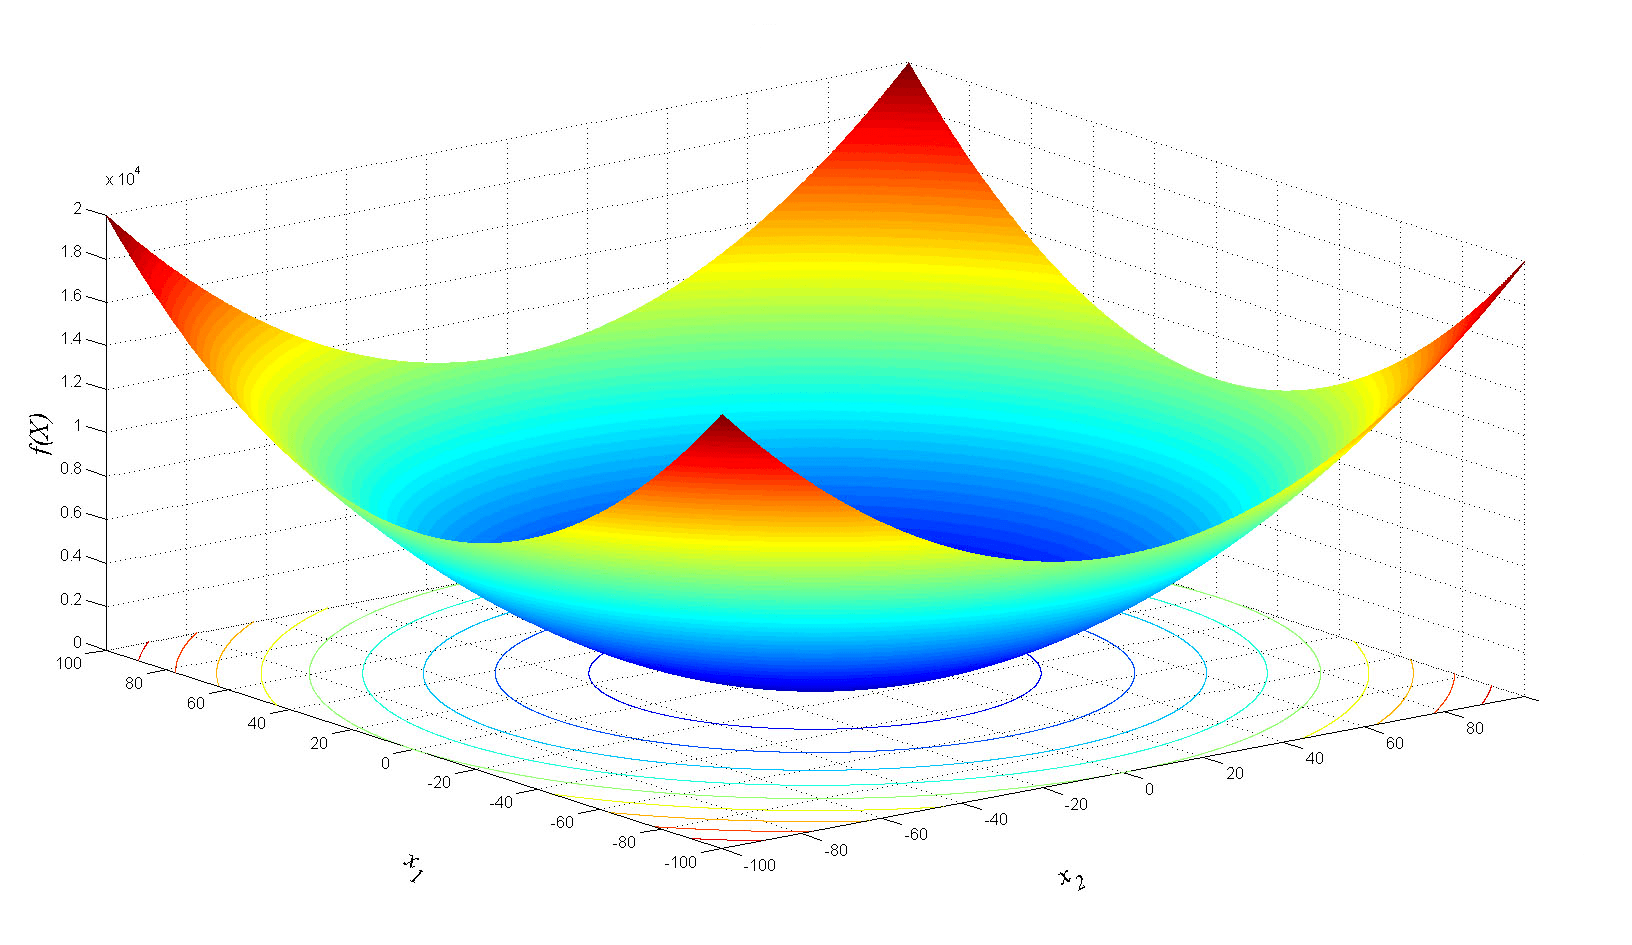
\includegraphics[width=100mm,scale=0.5]{De_Jong_function}
  \caption{Image De Jong's Function.\protect\footnotemark}
\end{figure}
\footnotetext{https://al-roomi.org/benchmarks/unconstrained/n-dimensions/}

\begin{figure}[!h]
  \centering
  $$ f(x) = \sum_{i=1}^n \left[-x_i \cdot sin(sqrt(|x_i|)) \right],
   x_i \in \left[ -500, 500 \right]$$

  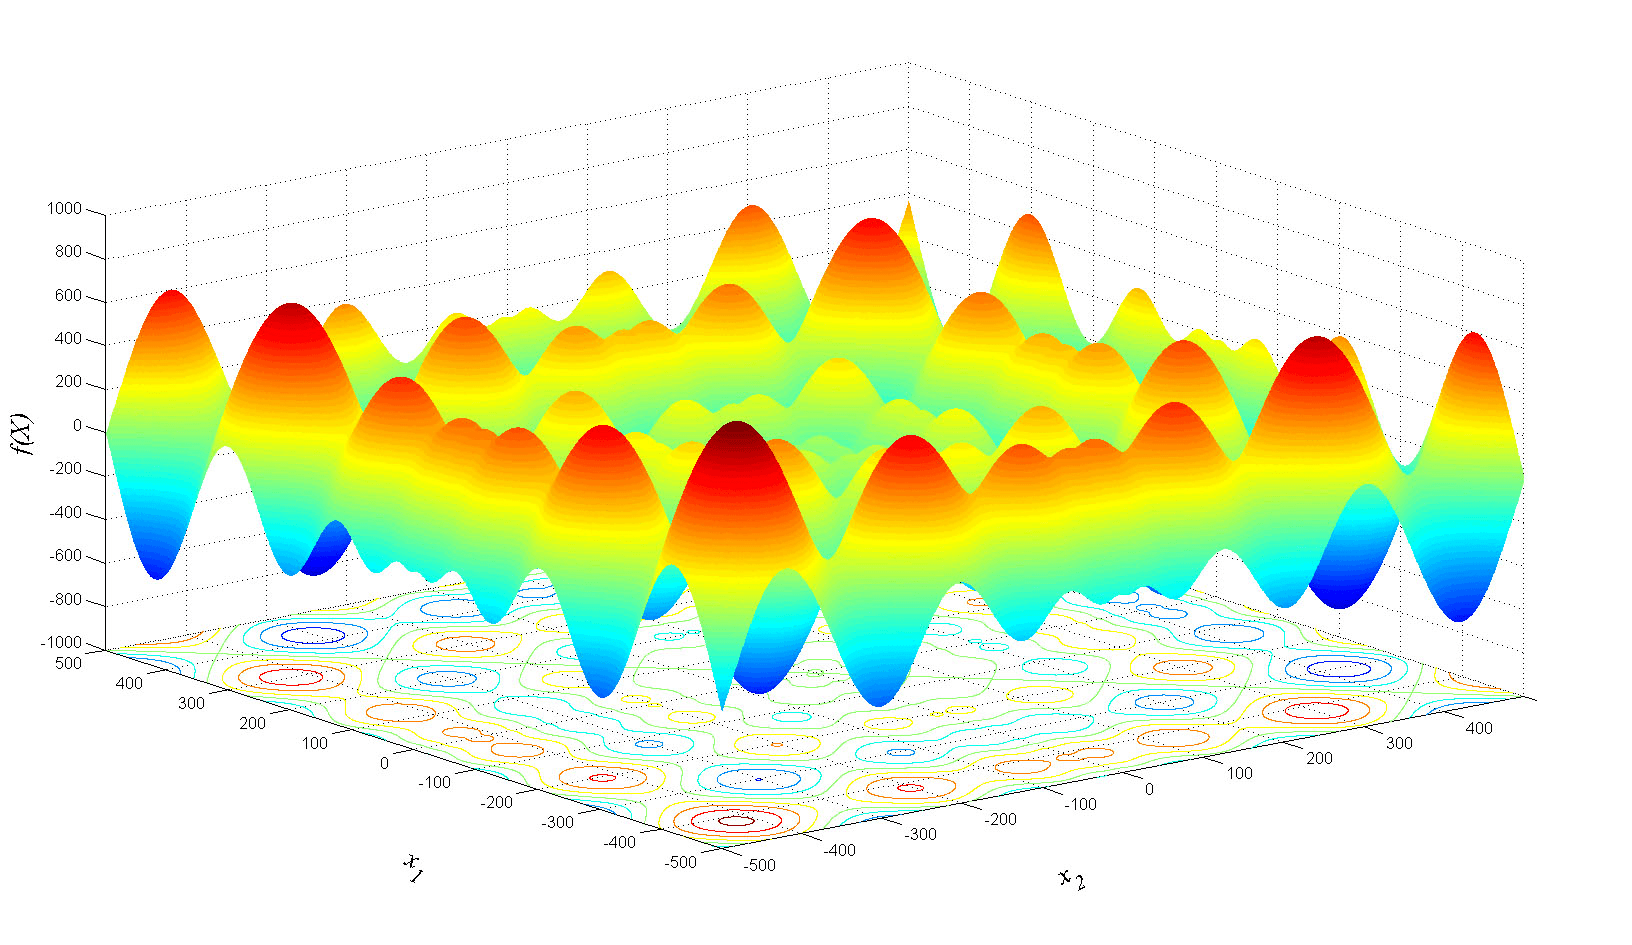
\includegraphics[width=100mm,scale=0.5]{Schwefel_fucntion}
  \caption{Image Schwefel's Function. \protect\footnotemark}
\end{figure}
\footnotetext{https://al-roomi.org/component/tags/tag/schwefel-function}

\begin{figure}[!h]
  \centering
  $$ f(x) = A \cdot n + \sum_{i=1}^n \left[ x_i^2 - A \cdot cos(2 \pi x_i) \right],
  A = 10, x_i \in \left[ -5.12, 5.15 \right]$$

  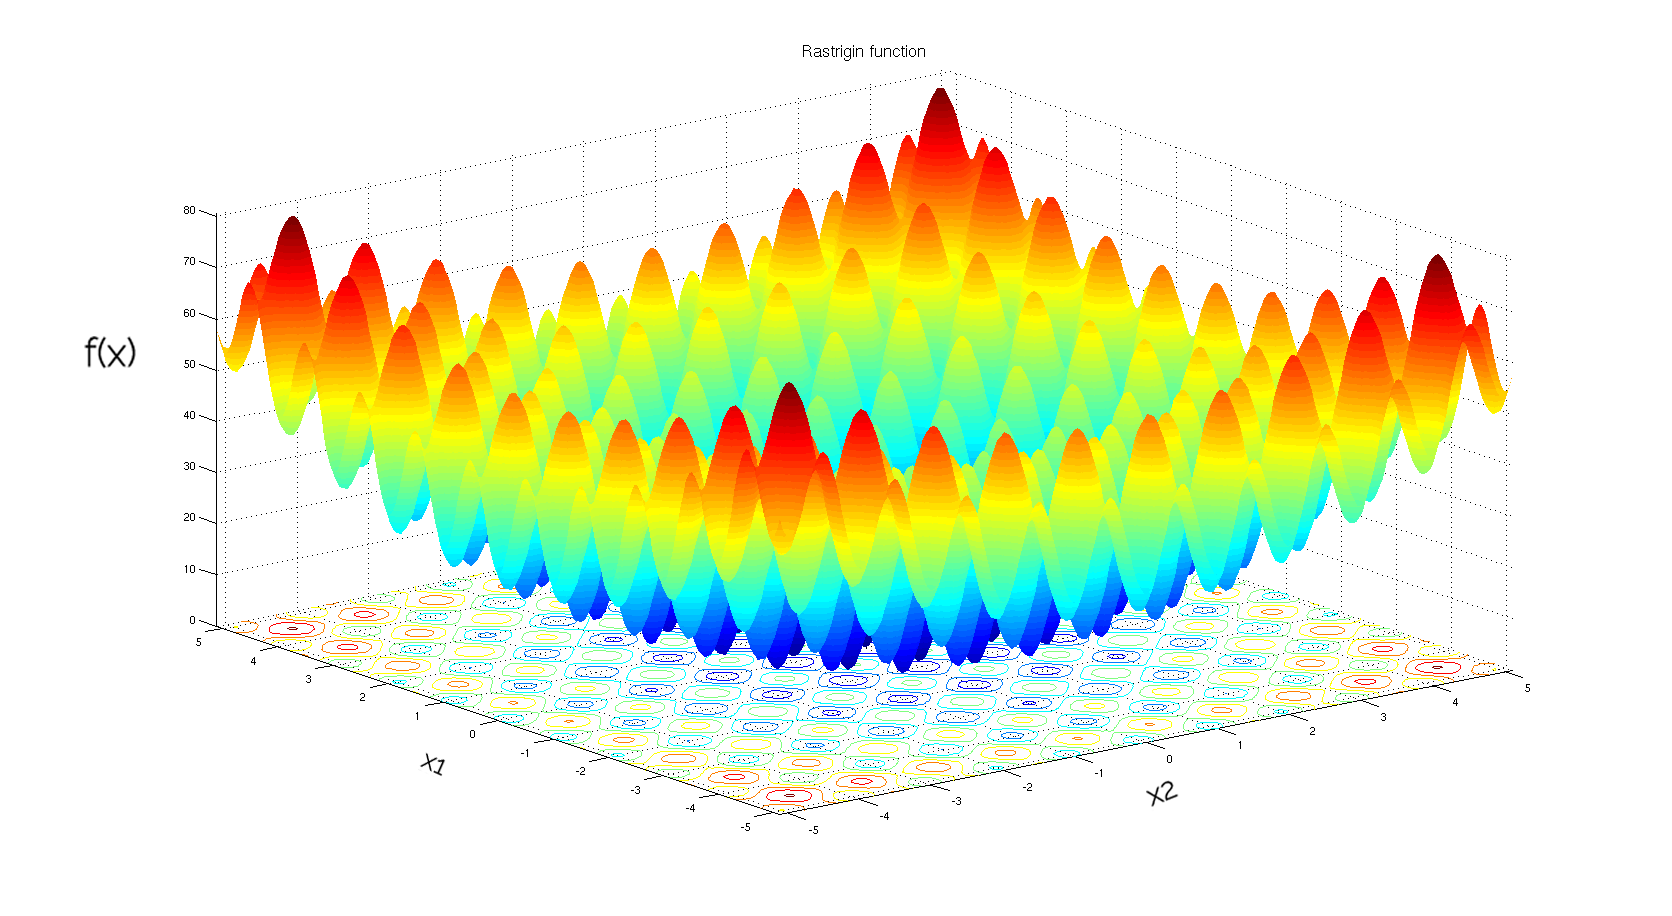
\includegraphics[width=100mm,scale=0.5]{Rastrigin_function}
  \caption{Image Rastrigin's Function. \protect\footnotemark}
\end{figure}
\footnotetext{https://commons.wikimedia.org/wiki/MainPage}

\begin{figure}[!h]
  \centering
  $$ f(x) = -\sum_{i=1}^n \left[sin(x_i) \cdot \left( sin\left( \frac{i \cdot x_i^2}{\pi}  \right) \right)^{2 \cdot m} \right] ,
  x_i \in \left[ 0, \pi \right] ,  m = 10$$

  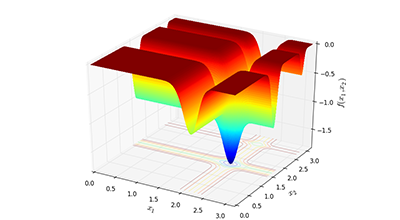
\includegraphics[width=100mm,scale=0.5]{Michalewicz_functions}
  \caption{Michalewicz's Function. \protect\footnotemark}
\end{figure}
\footnotetext{https://www.sfu.ca/~ssurjano/michal.html}

\pagebreak

\section{Results}

Hill Climbing first 5D
\newline
\newline
\begin{tabulary}{1\textwidth}{|c|c|c|c|c|}
\hline
\multirow{2}{*}{Functions} & \multicolumn{3}{c|}{Solutions} & \multirow{2}{*}{Time Averege}
     \\
\cline{2-4}
 & Averege & Minimum &  Maximum &  \\
\hline
 DeJong 1 & 0 & 0 & 0 & 14 \\
\hline
 Schwefel & -1939 & -1992 & -1853 & 22  \\
\hline
 Rastrigin & 2.29497 & 1.58367 & 3.39702 & 26  \\
\hline
 Michalewicz & -4.44109 & -4.62793 & -3.97123 & 22 \\
\hline
\end{tabulary}
\newline
\newline
Hill Climbing best 5D
\newline
\newline
\begin{tabulary}{1\textwidth}{|c|c|c|c|c|}
\hline
\multirow{2}{*}{Functions} & \multicolumn{3}{c|}{Solutions} & \multirow{2}{*}{Time Averege}
     \\
\cline{2-4}
 & Averege & Minimum &  Maximum &  \\
\hline
 DeJong 1 & 0 & 0 & 0 & 28 \\
\hline
 Schwefel & -1967 & -2094 & -1893 & 20 \\
\hline
 Rastrigin & 1.93592 & 1.279144 & 1.68702 & 28 \\
\hline
 Michalewicz & -4.37306 &  -4.65685 & -4.02012 & 20 \\
\hline
\end{tabulary}
\newline
\newline
Simulated Annealing 5D
\newline
\newline
\begin{tabulary}{1\textwidth}{|c|c|c|c|c|}
\hline
\multirow{2}{*}{Functions} & \multicolumn{3}{c|}{Solutions} & \multirow{2}{*}{Time Averege}
     \\
\cline{2-4}
 & Averege & Minimum &  Maximum &  \\
\hline
 DeJong 1 & 0 & 0 & 0 & 4 \\
\hline
 Schwefel & -1825 & -1963 & -1776  & 6  \\
\hline
 Rastrigin & 2.23086 & 1.71005 & 3.102193 & 6 \\
\hline
 Michalewicz & -4.28916 & -4.6328 & -3.26917 & 4 \\
\hline
\end{tabulary}
\newline
\newline
Hill Climbing first 10D
\newline
\newline
\begin{tabulary}{1\textwidth}{|c|c|c|c|c|}
\hline
\multirow{2}{*}{Functions} & \multicolumn{3}{c|}{Solutions} & \multirow{2}{*}{Time Averege}
     \\
\cline{2-4}
 & Averege & Minimum &  Maximum &  \\
\hline
 DeJong 1 & 0 & 0 & 0 & 112 \\
\hline
 Schwefel & -3652 & -3872 & -3492 & 262 \\
\hline
 Rastrigin & 7.18790 & 3.93217 & 15.19234 & 322 \\
\hline
 Michalewicz & -8.20880 & -9.01029 & -6.89132 & 214 \\
\hline
\end{tabulary}
\newline
\newline
Hill Climbing best 10D
\newline
\newline
\begin{tabulary}{1\textwidth}{|c|c|c|c|c|}
\hline
\multirow{2}{*}{Functions} & \multicolumn{3}{c|}{Solutions} & \multirow{2}{*}{Time Averege}
     \\
\cline{2-4}
 & Averege & Minimum &  Maximum &  \\
\hline
 DeJong 1 & 0 & 0 & 0 & 216 \\
\hline
 Schwefel & -3623 & -3772 & -3506 & 166 \\
\hline
 Rastrigin & 8.18790 & 3.67834 & 14.0925 & 242 \\
\hline
 Michalewicz & -9.09037 &  -9.24031 & -8.25910 & 158 \\
\hline
\end{tabulary}
\newline
\newline
Simulated Annealing 10D
\newline
\newline
\begin{tabulary}{1\textwidth}{|c|c|c|c|c|}
\hline
\multirow{2}{*}{Functions} & \multicolumn{3}{c|}{Solutions} & \multirow{2}{*}{Time Averege}
     \\
\cline{2-4}
 & Averege & Minimum &  Maximum &  \\
\hline
 DeJong 1 & 0 & 0 & 0 & 8 \\
\hline
 Schwefel & -3642 & -3905 & -3246  & 14 \\
\hline
 Rastrigin & 9.18790 & 3.19593 & 15.2394 & 14 \\
\hline
 Michalewicz & -8.70903 & -9.22690 &  -6.15737 & 12 \\
\hline
\end{tabulary}
\newline
\newline
Hill Climbing first 30D
\newline
\newline
\begin{tabulary}{1\textwidth}{|c|c|c|c|c|}
\hline
\multirow{2}{*}{Functions} & \multicolumn{3}{c|}{Solutions} & \multirow{2}{*}{Time Averege}
     \\
\cline{2-4}
 & Averege & Minimum &  Maximum &  \\
\hline
 DeJong 1 & 0 & 0 & 0 & 1946 \\
\hline
 Schwefel & -9453 & -9923 & -9369 & 3051 \\
\hline
 Rastrigin & 33.72184 & 27.12235 & 48.63187 & 3234 \\
\hline
 Michalewicz & -20.79776 & -22.61219 & -17.31592 & 1260 \\
\hline
\end{tabulary}
\newline
\newline
Hill Climbing best 30D
\newline
\newline
\begin{tabulary}{1\textwidth}{|c|c|c|c|c|}
\hline
\multirow{2}{*}{Functions} & \multicolumn{3}{c|}{Solutions} & \multirow{2}{*}{Time Averege}
     \\
\cline{2-4}
 & Averege & Minimum &  Maximum &  \\
\hline
 DeJong 1 & 0 & 0 & 0 & 2570 \\
\hline
 Schwefel & -10153 & -10453 & -10063 & 3022 \\
\hline
 Rastrigin & 32.43780 & 26.97201 & 47.29053 & 2784 \\
\hline
 Michalewicz & -24.09166 & -25.14376 & -22.21472 & 846 \\
\hline
\end{tabulary}
\newline
\newline
Simulated Annealing 30D
\newline
\newline
\begin{tabulary}{1\textwidth}{|c|c|c|c|c|}
\hline
\multirow{2}{*}{Functions} & \multicolumn{3}{c|}{Solutions} & \multirow{2}{*}{Time Averege}
     \\
\cline{2-4}
 & Averege & Minimum &  Maximum &  \\
\hline
 DeJong 1 & 0 & 0 & 0 & 20  \\
\hline
 Schwefel & -9746  & -11279 & -9365  & 40  \\
\hline
 Rastrigin & 35.18790 & 27.67834 & 56.44140 & 42  \\
\hline
 Michalewicz & -23.66259 & -24.29173 & -21.53991 & 30 \\
\hline
\end{tabulary}


\section{Conclusions}
In my resaults, Hill Climbing best improovement usualy gives slightly better resaults than first improovement while neither algorithm is clearly better in terms of time.
\newline
As expected, with larger input, the time increses significantly, and the difference between the minimum and the maximum is higher, which could simbolize a lower precission.
\newline
The resaults could be improoved by using a different random function and the time could be improoved by implmenting the program in C++ rather than Python.
\newline
In my implementation the Simulated Annealing algorithm, gives worse resaults than Hill Climbing with higher difference between the minimum and maximum, but the time is more than 10 times better, and the increese in input size doesn't increese the time at the same rate as the Hill Climbing. 
\newline
The algorithm could be improoved by using a better temperature function, and perhaps finding a way to make it more efficient at low temperatures.
\newline

As demonstrated in the experiment, nondeterministic algorithms can be used to find the global minimum of functions.


\begin{thebibliography}{9}

\bibitem{wikipedia}
  Wikipedia Commons \\ Rastrigin's Function rendered image.
  \url{https://commons.wikimedia.org/wiki/Main_Page}

\bibitem{Al-roomi}
  Al-roomi  \\ De Jong's Function rendered image.
  \url{https://al-roomi.org/benchmarks/unconstrained/n-dimensions/}
  Al-roomi  \\ Schwefel's Function rendered image.
  \url{https://al-roomi.org/component/tags/tag/schwefel-function}

\bibitem{Sfui}
   Sfu \\ Michalewicz's Function rendered image.  
\url{https://www.sfu.ca/~ssurjano/michal.html}


\bibitem{Geatbx}
  Geatbxi  \\ Function formulas.
  \url{http://www.geatbx.com/docu/fcnindex-01.html}

\bibitem{Course}
  Course Page.
  \url{https://profs.info.uaic.ro/~eugennc/teaching/ga/l}

\bibitem{Pycharm}
  Pycharm.
  \url{https://www.jetbrains.com/pycharm/}


\end{thebibliography}  
\end{document}
